\documentclass[margin=2cm]{standalone}

\usepackage{tikz,xcolor}

\usetikzlibrary{intersections,shapes.arrows,calc}

\definecolor{lgray}{cmyk}{0,0,0,0.2}
\definecolor{dgray}{cmyk}{0,0,0,0.7}



\tikzset
{
    % Style for the intersecting path, which are necessary for the calculation but
    % shouldn't be drawn in the final image
    ipath/.style=
    {
        draw, % comment this out after construction
        red
    },
    % Style for an arrow used as object
    optical arrow/.style=
    {
        fill=dgray,
        inner sep=3pt,
        shape=single arrow,
        minimum width=0.5cm,
        minimum height=1.5cm,
        outer sep=0pt,
        shape border rotate=90
    },
    % Style for the virtual image
    virtual optical arrow/.style=
    {
        fill=lgray,
        inner sep=3pt,
        shape=single arrow,
        minimum width=0.5cm,
        minimum height=1.5cm,
        outer sep=0pt,
        shape border rotate=90
    },
    % Style for the mirror
    mirror/.style=
    {
        line width=2pt
    },
    %Style for the axis
    optical axis/.style=
    {
        thin
    },
    % Style for light rays
    ray/.style=
    {
        thin,
        ->
    },
    % Style for imagined rays, thich are not real but help by constructing the image
    imagined ray/.style=
    {
        ray,
        dgray,
        -
    },
    % Alias
    virtual ray/.style={imagined ray},
    % Style for (focal) points
    point/.style=
    {
        fill=black,
        radius=0.8pt,
        inner sep=1pt,
        shape=circle,
        minimum size=2pt,
        outer sep=2pt
    }
}

% Set three layers
\pgfdeclarelayer{background}
\pgfdeclarelayer{foreground}
\pgfsetlayers{background,main,foreground}
% Define shortcuts to access them
\newcommand{\bglayer}[1]
{
    \begin{pgfonlayer}{background}
    #1
    \end{pgfonlayer}
}
\newcommand{\fglayer}[1]
{
    \begin{pgfonlayer}{foreground}
    #1
    \end{pgfonlayer}
}

\begin{document}



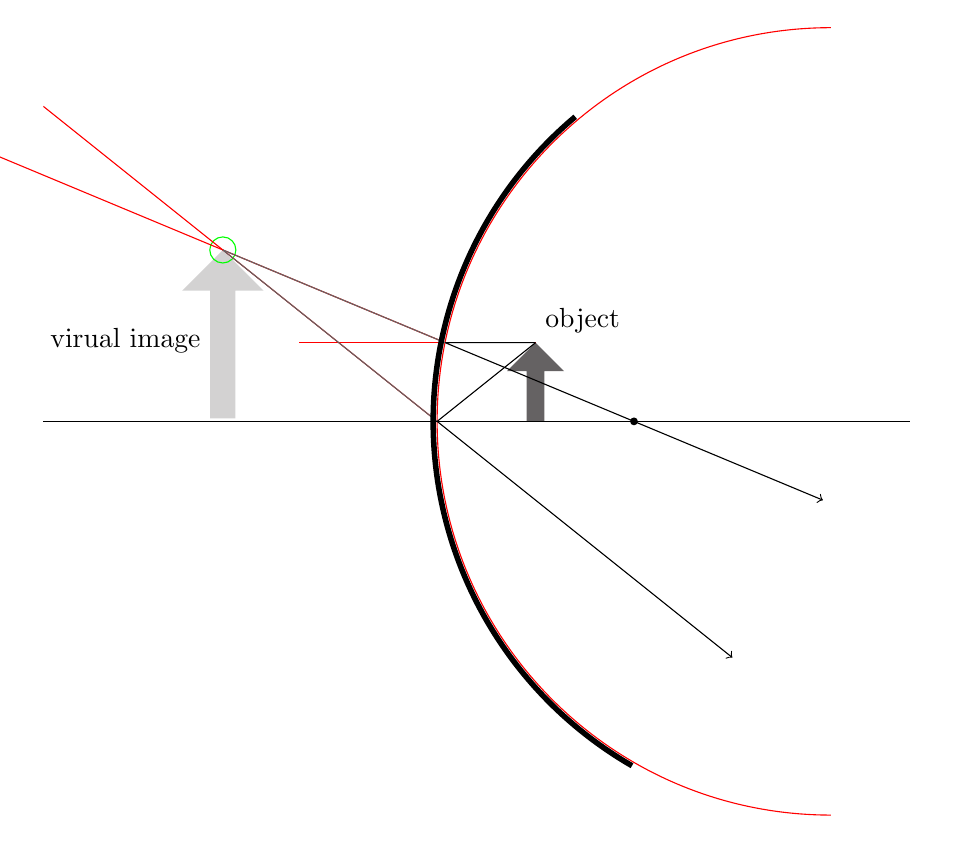
\begin{tikzpicture}
    % Define the bounding box. It's necessary because the ipaths make it bigger than needed
    \path [use as bounding box] (-5.2,-5) rectangle (6.2,5);

    % Define variables, you may vary them a little
    %% Radius
    \def\radius{5}
    \def\radiusII{5.05}
    %% Focal distance = \radius/2
    \def\focal{2.5}
    %% Object size
    \def\size{1cm}
    %% Object width
    \def\owidth{1.25}

    \coordinate (origin) (0,0);
    
    % % Extra for me to understand where everything is
    % \node at (0,0) [circle,draw,thick] {};
    % \node at (\radius,0) [circle,draw,blue,thick] {};

    % Draw mirror
    %% The extra ipath is necessary to get nicer rays
    \path [ipath, name path=M] (\radius,0) ++(90:\radius) arc (90:270:\radius);
    \fglayer
    {
        \draw[mirror] (\radiusII-0.05,0) ++(130:\radiusII) arc (130:240:\radiusII);
    }
    
    % Draw focal point
    \node (B) at (\focal,0) [point] {};

    % Draw object
    \node (O) [optical arrow,anchor=south,minimum height=\size] at (\owidth,0) {}; 
    %% Description
    \node at (O.north) [above right] {object};

    % Rays
    %% Draw axis ray
    \draw[ray] (O.north) -- (origin) -- ($(origin)!3!(\owidth,-\size)$);
    %% Draw parallel ray
    \path[ipath] [name path=PS] (O.north) -- ++(-3,0);
    \path [name intersections={of=M and PS, by=M-PS}];
    \draw[ray] (O.north) -- (M-PS) -- ($(M-PS)!2!(B)$);
    %% Calculate virtual axis ray
    \path[ipath] [name path=AS-V] ($(origin)!-4!(\owidth,-\size)$) -- (origin);
    %% Calculate virtual parallel ray
    \path[ipath] [name path=PS-V] ($(M-PS)!-4!(B)$) -- (M-PS);
    %% Draw virtual axis ray
    \path [name intersections={of=AS-V and PS-V, by={Tip-V}}];
    \draw[imagined ray] (Tip-V) -- (origin);
    %% Draw virtual axis ray
    \draw[imagined ray] (Tip-V) -- (M-PS);

    % Draw virtual object
    \bglayer
    {
        \path let \p{1}=(Tip-V) in
            (Tip-V) node (V) [minimum height=\size,
                              scale={\y{1}/\size*0.655},
                              virtual optical arrow,
                              anchor=tip] {}
                              node (0,\y{1}) [green,circle,draw] {};
    }
    %% description
    \path (V.west) node [left] {virual image};
    
    % Draw optical axis
    \fglayer
    {
        \draw[optical axis] (-5,0) -- +(11,0);
    }
    
\end{tikzpicture}


\end{document}